\chapter{Metodologia}
\label{chap:metodologia}

\lipsum[2]
\lipsum[12]

O autor \cite{lamport1986latex} e \cite{Maia2011} \lipsum[2] 

\begin{table}[h!]
	\Caption{\label{tabela-ibge} Um Exemplo de tabela alinhada que pode ser longa ou curta, conforme padrão IBGE. conforme padrão IBGE. conforme padrão IBGE. conforme padrão IBGE. conforme padrão IBGE. conforme padrão IBGE. conforme padrão IBGE. conforme padrão IBGE. conforme padrão IBGE. conforme padrão IBGE. conforme padrão IBGE.}%
	\IBGEtab{}{%
		\begin{tabular}{ccc}
			\toprule
			Nome & Nascimento & Documento \\
			\midrule %\midrule
			Maria da Silva & 11/11/1111 & 111.111.111-11 \\
			Maria da Silva & 11/11/1111 & 111.111.111-11 \\
			Maria da Silva & 11/11/1111 & 111.111.111-11 \\
			\bottomrule
		\end{tabular}%
	}{%
	\Fonte{Produzido pelos autores}%
	\Nota{Esta éuma nota, que diz que os dados são baseados na
		regressão linear.}%
	\Nota[Anotações]{Uma anotação adicional, seguida de várias outras.}%
}
\end{table}

\cite{Huetal2000} \lipsum[2] 

\section{Exemplo de Algoritmos e Figuras}
\label{sec:exemplo-de-algoritmos-e-figuras}

\lipsum[2]

\begin{algorithm}[h!]
	\SetSpacedAlgorithm
	\caption{\label{exemplo-de-algoritmo}Como escrever algoritmos no \LaTeX2e}
	\Entrada{o proprio texto}
	\Saida{como escrever algoritmos com \LaTeX2e }
	\Inicio{
		inicializa\c{c}\~ao\;
		\Repita{fim do texto}{
			leia o atual\;
			\Se{entendeu}{
				vá para o próximo\;
				próximo se torna o atual\;}
			\Senao{volte ao início da seção\;}
		}
	}	
\end{algorithm}

\lipsum[2]
%\begin{algorithm}[H]
%	\Entrada{o proprio texto}
%	\Saida{como escrever algoritmos com \LaTeX2e }
%	\Inicio{
%		inicializa\c{c}\~ao\;
%		\Repita{fim do texto}{
%			leia o atual\;
%			\Se{entendeu}{
%				vá para o próximo\;
%				próximo se torna o atual\;}
%			\Senao{volte ao início da seção\;}
%		}
%	}
%	\caption{Exemplo de Algoritmo Versao 02}
%\end{algorithm}

%\begin{algorithm}
%	\begin{algorithmic}
%	\Entrada{o proprio texto}
%	\Saida{como escrever algoritmos com \LaTeX2e }	
%	\end{algorithmic}
%\end{algorithm}

Exemplo de alíneas com números:

\begin{alineascomnumero}
	\item Lorem ipsum dolor sit amet, consectetur adipiscing elit. Nunc dictum sed tortor nec viverra.
	\item Praesent vitae nulla varius, pulvinar quam at, dapibus nisi. Aenean in commodo tellus. Mauris molestie est sed justo malesuada, quis feugiat tellus venenatis.
	\item Praesent quis erat eleifend, lacinia turpis in, tristique tellus. Nunc dictum sed tortor nec viverra.
	\item Mauris facilisis odio eu ornare tempor. Nunc dictum sed tortor nec viverra.
	\item Curabitur convallis odio at eros consequat pretium.
\end{alineascomnumero}

\lipsum[12]

\begin{table}[h!]	
	\centering
	\Caption{\label{tab:internal}Internal exon scores}	
	\IBGEtab{}{
		\begin{tabular}{cll}
			\toprule
			Ranking & Exon Coverage & Splice Site Support\\
			\midrule \midrule
			E1 & Complete coverage by a single transcript & Both splice sites\\
			E2 & Complete coverage by more than a single transcript & Both splice sites\\
			E3 & Partial coverage & Both splice sites\\
			E4 & Partial coverage & One splice site\\
			E5 & Complete or partial coverage & No splice sites\\
			E6 & No coverage & No splice sites\\
			\bottomrule
		\end{tabular}
	}{
	\Fonte{os autores}
}
\end{table}

\lipsum[2] Referenciando a \autoref{tab:internal} \lipsum[2]

\index{figuras}Figuras podem ser criadas diretamente em LaTeX,
como o exemplo da \ref{fig-grafico-1}.

\begin{figure}[h!]
	\centering
	\Caption{\label{fig-grafico-1}Produção anual das dissertações de mestrado e teses de doutorado entre os anos de 1990 e 2008}		
	\IBGEtab{}{
		\fbox{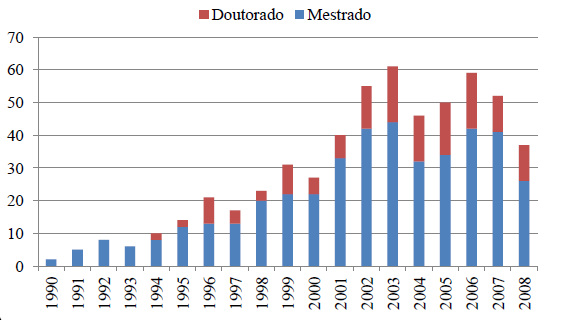
\includegraphics[scale=0.5]{figuras/figura-3}}
	}{
	\Fonte{os autores}
}
\end{figure}

Ou então figuras podem ser incorporadas de arquivos externos, como é o caso da \autoref{fig-grafico-1}. Se a figura que ser incluída se tratar de um diagrama, um gráfico ou uma ilustração que você mesmo produza, priorize o uso de imagens vetoriais no formato PDF. Com isso, o tamanho do arquivo final do trabalho será menor, e as imagens terão uma apresentação melhor, principalmente quando impressas, uma vez que imagens vetorias são perfeitamente escaláveis para qualquer dimensão. Nesse caso, se for utilizar o Microsoft Excel para produzir gráficos, ou o Microsoft Word para produzir ilustrações, exporte-os como PDF e os incorpore ao documento conforme o exemplo abaixo. No entanto, para manter a coerência no uso de software livre (já que você está usando LaTeX e abnTeX),  teste a ferramenta InkScape\index{InkScape}. ao CorelDraw\index{CorelDraw} ou ao Adobe Illustrator\index{Adobe! Illustrator}.  De todo modo, caso não seja possível  utilizar arquivos de imagens como PDF, utilize qualquer outro formato, como JPEG, GIF, BMP, etc.  Nesse caso, você pode tentar aprimorar as imagens incorporadas com o software livre \index{Gimp}Gimp. Ele é uma alternativa livre ao Adobe Photoshop\index{Adobe! Photoshop}.

\section{Usando Fórmulas Matemáticas}

\lipsum[2]

	\begin{equation}
		\begin{aligned}
			x = a_0 + \cfrac{1}{a_1
				+ \cfrac{1}{a_2
					+ \cfrac{1}{a_3 + \cfrac{1}{a_4} } } }
		\end{aligned}
	\end{equation}

\lipsum[3]

	\begin{equation}
		\begin{aligned}
			k_{n+1} = n^2 + k_n^2 - k_{n-1}
		\end{aligned}
	\end{equation}

\lipsum[4]

	\begin{equation}
		\begin{aligned}
			\cos (2\theta) = \cos^2 \theta - \sin^2 \theta
		\end{aligned}
	\end{equation}
	
\lipsum[5]

	\begin{equation}
		\begin{aligned}
			A_{m,n} =
			\begin{pmatrix}
			a_{1,1} & a_{1,2} & \cdots & a_{1,n} \\
			a_{2,1} & a_{2,2} & \cdots & a_{2,n} \\
			\vdots  & \vdots  & \ddots & \vdots  \\
			a_{m,1} & a_{m,2} & \cdots & a_{m,n}
			\end{pmatrix}
		\end{aligned}
	\end{equation}

\lipsum[6]

	\begin{equation}
		\begin{aligned}
			f(n) = \left\{ 
			\begin{array}{l l}
			n/2 & \quad \text{if $n$ is even}\\
			-(n+1)/2 & \quad \text{if $n$ is odd}
			\end{array} \right.
		\end{aligned}
	\end{equation}
	
\lipsum[7]

\section{Usando Algoritmos}

\lipsum[8]

\begin{algorithm}[h!]
	\SetSpacedAlgorithm
	\caption{\label{alg:algoritmo_de_colonica_de_formigas}Algoritmo de Otimização por Colônia de Formiga}
	\Entrada{Entrada do Algoritmo}
	\Saida{Saida do Algoritmo}
	\Inicio{
		Atribua os valores dos parâmetros\;
		Inicialize as trilhas de feromônios\;
		\Enqto{não atingir o critério de parada}{
			\Para{cada formiga}{
				Construa as Soluções\;
			}
			Aplique Busca Local (Opcional)\;
			Atualize o Feromônio\;
		}	
	}		
\end{algorithm}

\lipsum[9]

\section{Usando Código-fonte}

\lipsum[10]

\lstinputlisting[language=C++,caption={Hello World em C++}]{figuras/main.cpp}

\lipsum[11]

\begin{lstlisting}[language=Java,caption={Hello World em Java}]
public class HelloWorld {
	public static void main(String[] args) {
		System.out.println("Hello World!");
	}
}
\end{lstlisting}

\lipsum[11]

\section{Usando Teoremas, Proposições, etc}

Lorem ipsum dolor sit amet, consectetur adipiscing elit. Nunc dictum sed tortor nec viverra. consectetur adipiscing elit. Nunc dictum sed tortor nec viverra.

\begin{teo}[Pitágoras]
	Em todo triângulo retângulo o quadrado do comprimento da
	hipotenusa é igual a soma dos quadrados dos comprimentos dos catetos.
\end{teo}


Lorem ipsum dolor sit amet, consectetur adipiscing elit. Nunc dictum sed tortor nec viverra. consectetur adipiscing elit. Nunc dictum sed tortor nec viverra.

\begin{teo}[Fermat]
	Não existem inteiros $n > 2$, e $x, y, z$ tais que $x^n + y^n = z$
\end{teo}

Lorem ipsum dolor sit amet, consectetur adipiscing elit. Nunc dictum sed tortor nec viverra. consectetur adipiscing elit. Nunc dictum sed tortor nec viverra.

\begin{prop}
	Para demonstrar o Teorema de Pitágoras...
\end{prop}

Lorem ipsum dolor sit amet, consectetur adipiscing elit. Nunc dictum sed tortor nec viverra. consectetur adipiscing elit. Nunc dictum sed tortor nec viverra.

\begin{exem}
	Este é um exemplo do uso do ambiente exe definido acima.
\end{exem}

Lorem ipsum dolor sit amet, consectetur adipiscing elit. Nunc dictum sed tortor nec viverra. consectetur adipiscing elit. Nunc dictum sed tortor nec viverra.

\begin{xdefinicao}
	Definimos o produto de ...
\end{xdefinicao}

Lorem ipsum dolor sit amet, consectetur adipiscing elit. Nunc dictum sed tortor nec viverra. consectetur adipiscing elit. Nunc dictum sed tortor nec viverra.

\section{Usando Questões}


Lorem ipsum dolor sit amet, consectetur adipiscing elit. Nunc dictum sed tortor nec viverra. consectetur adipiscing elit. Nunc dictum sed tortor nec viverra.

\begin{questao}
	\item Esta é a primeira questão com alguns itens:
		\begin{enumerate}
			\item Este é o primeiro item
			\item Segundo item
		\end{enumerate}
	\item Esta é a segunda questão:
		\begin{enumerate}
			\item Este é o primeiro item
			\item Segundo item
		\end{enumerate}
	\item Lorem ipsum dolor sit amet, consectetur adipiscing elit. Nunc dictum sed tortor nec viverra. consectetur adipiscing elit. Nunc dictum sed tortor nec viverra.
		\begin{enumerate}
			\item consectetur
			\item adipiscing
			\item Nunc
			\item dictum
		\end{enumerate}
\end{questao}

\section{Citações}

\subsection{Documentos com três autores}

Quando houver três autores na citação, apresentam se os três, separados por ponto e vírgula, caso estes estejam após o texto. Se os autores estiverem incluídos no texto, devem ser separados por vírgula e pela conjunção "e".

\citeautoronline{tresautores}

\cite{tresautores}

\subsection{Documentos com mais de três autores}
Havendo mais de três autores, indica-se o primeiro seguido da expressão \textit{et al.} (do latim \textit{et alli}, que significa e outros), do ano e da página.

\citeautoronline{quatroautores}

\cite{quatroautores}

\cite{kurose2013}

\cite{pinheiro2004site}

\cite{costa1998}

\cite{gorshe2014ieee}

\citeautoronline{cartilhaUCAredessemfio}

\cite{moraes2014}

\cite{amer2016acm}

\cite{tanenbaum2013}

\cite{rodrigues2007site}

\cite{marconi2017}

\cite{gil2002}

\cite{barbosa2012}

\cite{wiki}

\subsection{Documentos de vários autores}

Havendo    citações    indiretas de    diversos    documentos    de    vários    autores, mencionados  simultaneamente e  que  expressam  a  mesma  ideia,  separam-se  os  autores  por ponto e vírgula, em ordem alfabética.

\cite{tresautores, quatroautores}

\section{Notas de Rodap\'{e}}

%Deve-se utilizar o sistema autor-data para as  citações no texto e o numérico para notas explicativas\footnote{Veja - se como exemplo desse tipo de abordagem o estudo de Netzer (1976)}. As notas de rodapé podem e devem ser alinhadas, a partir da segunda linha da mesma nota, abaixo da primeira letra da primeira palavra, de forma a destacar o expoente \footnote{Encontramos  esse  tipo  de  perspectiva  na  2ª  parte  do  verbete  referido  na  nota  anterior,  em  grande  parte  do estudo de Rahner (1962).} e sem espaço entre elas e com fonte menor (tamanho 10).

